\section{mo\-Cooling\-Schedule Class Reference}
\label{classmo_cooling_schedule}\index{moCoolingSchedule@{moCoolingSchedule}}
This class gives the description of a cooling schedule.  


{\tt \#include $<$mo\-Cooling\-Schedule.h$>$}

Inheritance diagram for mo\-Cooling\-Schedule::\begin{figure}[H]
\begin{center}
\leavevmode
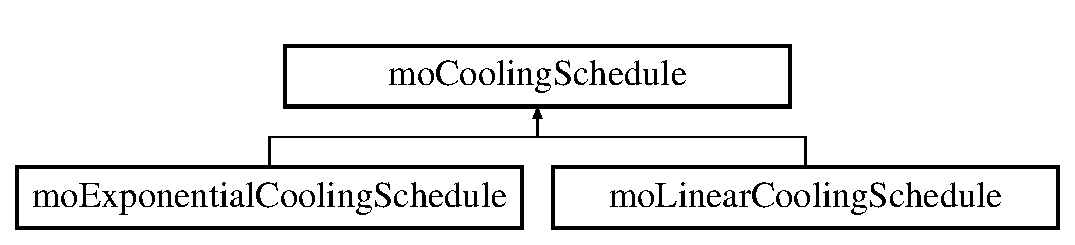
\includegraphics[height=4cm]{classmo_cooling_schedule}
\end{center}
\end{figure}


\subsection{Detailed Description}
This class gives the description of a cooling schedule. 

It is only a description... An object that herits from this class is needed to be used in a {\bf mo\-SA}{\rm (p.\,\pageref{classmo_s_a})}. See {\bf mo\-Exponential\-Cooling\-Schedule}{\rm (p.\,\pageref{classmo_exponential_cooling_schedule})} or {\bf mo\-Linear\-Cooling\-Schedule}{\rm (p.\,\pageref{classmo_linear_cooling_schedule})} for example. 



Definition at line 46 of file mo\-Cooling\-Schedule.h.

The documentation for this class was generated from the following file:\begin{CompactItemize}
\item 
mo\-Cooling\-Schedule.h\end{CompactItemize}
